% O problema de N-corpos (PNC) consiste de um sistema mecânico cujo movimento é descrito por um sistema de equações diferenciais ordinárias de segunda ordem, cuja solução tem existência local garantida no espaço euclidiano sem as singularidades (VOLCHAN). O PNC tem algumas propriedades imanentes garantidas por qualquer potencial V_k de grau k, como: energia total, momento linear total, momento angular total, centro de massas (integrais primeiras), redimensionamento e momento de inércia, o que fornece também duas relações interessantes: a relação de Distanciamentos e a relação de Lagrange-Jacobi (VOLCHAN). Formas de lidar com singularidades: regularização para colisões binárias; adicionando colisões elásticas para testar.

\chapter{O Problema de N-Corpos Gravitacional}\label{capitulo:pncg}

O Problema de N-Corpos Gravitacional (PNCG) é um sistema mecânico descrito por um conjunto de equações diferenciais ordinárias de segunda ordem, com existência e unicidade de solução garantidas localmente pelo Teorema de Existência de Unicidade. O PNCG possui algumas propriedades inerentes garantidas por seu potencial homogêneo, como a presença de uma integral primeira escalar e outras três vetoriais, a semelhança de soluções pelo redimensionamento anisotrópico, medidas de distanciamento e evolução da expansão.

Este capítulo é dedicado ao estudo do PNCG e de suas propriedades básicas citadas, sem, no entanto, se focar em questões demasiado específicas, como soluções analíticas para problemas de dois ou três corpos. São apresentados conceitos e propriedades gerais, além de uma introdução à Dinâmica de Formas sob o \textit{toy-model} de N-corpos.


\section{Enunciado}
Considere um conjunto de $N$ partículas dispostas no vácuo tridimensional ($\R^3$, digamos), cada uma com massa $m_a$, posição $\vet q_a$ e velocidade $\vet v_a$, para $a = 1, 2, ..., N$. A \textit{Lei da Gravitação Universal de Newton} fornece a seguinte função potencial suave:
\begin{equation}\label{eq:potencial_newtoniano}
    V = - \sum_{a < b} G \dfrac{m_a m_b}{r_{ab}},
    \quad
    r_{ab} = \norma{\vet q_a - \vet q_b},
\end{equation}
onde $G$ é a \textit{constante de gravitação universal}.

A partir de $V$, define-se um campo gradiente $\vet F = - \nabla V$ que gera as seguintes equações de movimento, conforme (\ref{eq:segunda_lei_de_newton}):
\begin{equation}\label{eq:mov_gravitacao}
    \begin{cases}
        \dvet q_a = \vet v_a, \\
        \dvet v_a = \dfrac{1}{m_a} \vet F_a = \sum_{b \neq a}^N G m_b \dfrac{\vet q_b - \vet q_a}{r_{ab}^3},
    \end{cases}
        \quad \forall a = 1, 2, ..., N.
\end{equation}

A existência e a unicidade das soluções das equações (\ref{eq:mov_gravitacao}) munidas de um conjunto de valores iniciais é garantida localmente em $(\R^3 / \Delta) \times \R^3$ pelo \textit{Teorema de Existência e Unicidade}, cuja demonstração pode ser encontrada em \citep[34-36]{Volchan:2007}. Aqui, $\Delta$ é o \textit{conjunto singular}, dado por
\begin{equation*}
    \Delta = \bigcup_{1 \leq i < j \leq N} \{(\vet q_1, ..., \vet q_N) \in \R^{3N}: \vet q_i = \vet q_j \}.
\end{equation*}

Observe que também é possível representar o problema em termos de posições e momentos conjungados, tomando $\vet p_a = m_a \vet q_a, \forall a$ e escrevendo as equações de Hamilton:
\begin{equation}
    \begin{cases}
        \dvet q_a = \derpar{H}{\vet p_a} = - \vet p_a / m_a, \\
        \dvet p_a = - \derpar{H}{\vet q_a} = \sum_{b \neq a}^N G m_a m_b \dfrac{\vet q_b - \vet q_a}{r_{ab}^3},
    \end{cases}
\end{equation}
onde como função Hamiltoniana toma-se a energia total:
\begin{equation*}
    H (\vet q, \vet p) = T(\vet p) + V(\vet q).
\end{equation*}

\section{Integrais primeiras}
O PNCG tridimensional possui dez integrais primeiras, cada uma correspondente a uma simetria dentro do sistema.

\begin{theorem}
    O PNCG possui como integrais primeiras não-triviais a energia total $E$ (correspondente à invariância temporal), momento angular total $\vet J$ (correspondente à invariância sob rotações), o momento linear total $\vet P$ e a trajetória $\vet G(t)$ do centro de massas $\vet q_{cm}$ (correspondentes à invariância sob translações).
\end{theorem}
\begin{Proof}
    Para a energia total, a demonstração já foi feita no Teorema \ref{teorema:energia_total}.

    Para o momento linear total $\vet P = \sum_{a=1}^N \vet p_a$, basta aplicar a definição \ref{def:integral_primeira}:
    \begin{equation*}
        \der{\vet P}{t} = \sum_{a=1}^{N} \der{\vet p_a}{t} = \sum_{a=1}^N \vet F_a = \vet 0,
    \end{equation*}
    pois o sistema é fechado.

    Para a trajetória do centro de massas, temos:
    \begin{equation}
        \vet G(t) = M \vet q_{cm} - t \vet P
        \Rightarrow
        \der{G}{t} = M \dfrac{\vet P}{M} - \vet P = \vet 0.
    \end{equation}
    No caso em que $\vet P = \vet 0$, a conservação de $G(t)$ equivale à conservação de $\vet q_{cm}$.

    Por fim, o momento angular total:
    \begin{equation}
        \der{\vet J}{t} 
        = \sum_{a=1}^N \vet q_a \times \dvet p_a
        = \sum_{a=1}^N \sum_{b\neq a}^{N} \dfrac{G m_a m_b}{r_{ab}^3} \vet q_a \times \vet q_b = \vet 0.
    \end{equation}
\end{Proof}

O fato de o centro de massas do Problema ter uma rota linear e seu momento generalizado ($\vet P$) ser uma integral primeira significa que se o centro de massas partir da origem e o momento linear total for nulo, o sistema não deverá se mover. Isso é particularmente interessante para simulações numéricas, mas mesmo analiticamente ainda é uma propriedade que facilita o estudo.

\section{Questões de escala}
Nas simulações numéricas diretas de gravitação (ou seja, integrando diretamente as equações de movimento do PNCG), uma questão fundamental que aparece é a da escolha de unidades de medida padrão, de modo a garantir que diferentes simulações possam ser comparáveis. Alguns padrões foram definidos por \cite{aarseth_gravitational_2003} e são aplicados nos códigos NBODY \citep{NBODY}, e serão vistos com mais cuidados na seção de simulação. Para fins teóricos, a princípio, é possível obter algumas relações acerca da medida dos sistemas de partículas e das órbitas.

Para começar, para cada problema de valor inicial do PNCG, é possível obter uma família infinita de órbitas idênticas a menos de um fator de escala anisotrópico. Isso significa que através de uma aplicação linear contínua, soluções são enviadas em soluções.

\begin{theorem}[Similaridade dinâmica]\label{teorema:similaridade_dinamica}
    As equações de movimento do PNCG satisfazem a similaridade dinâmica: se $(\vet q(t), \vet p(t))$ são órbitas do problema de N-corpos, o redimensionamento anisotrópico
    \begin{equation*}
        \tilde{\vet q}(\tilde t) = \alpha \vet q (t),
        \quad
        \tilde t = \alpha^{3/2} t,
        \quad
        \alpha > 0
    \end{equation*}
    das distâncias e do tempo newtoniano leva soluções $(\vet q(t), \vet p(t))$ em soluções $(\tilde{\vet q}(\tilde t), \tilde{\vet p}(\tilde t))$.
\end{theorem}
\begin{Proof}
    Considere um potencial geral homogêneo de grau $k$ e a mudança de coordenadas $\tilde{\vet q_a} = \alpha \vet q_a$, que implica em $\tilde t = \beta t$, para algum $\beta$ e então $\tilde{\vet p_a} = \alpha \vet p_a / \beta$. Com as novas coordenadas, temos a energia total
    \begin{equation*}
        H(\beta t, \alpha \vet q, \alpha \vet p / \beta) = \dfrac{\alpha^2}{\beta^2} T(\vet p) + \alpha^k V(\vet q).
    \end{equation*}
    Os sistemas são similarmente dinâmicos se $\beta$ for tal que podemos escrever $H(\tilde t, \tilde{\vet q}, \tilde{\vet p}) = \alpha^k H(t, \vet q, \vet p)$ (pois soluções são enviadas em soluções pelo redimensionamento). Decorre então que
    \begin{equation*}
        \alpha^k = \dfrac{\alpha^2}{\beta^2} \Rightarrow \beta = \alpha^{1-k/2}.
    \end{equation*}
    No PNCG temos que $k=-1$, e portanto $\tilde{\vet q_a} = \alpha \vet q_a$, $\tilde{\vet p_a} = \alpha^{-1/2} \vet p_a$ e $\tilde t = \alpha^{3/2} t$.
\end{Proof}

Observe que num problema de 2 corpos no qual um se encontra fixado e o outro sob uma órbita elíptica, se tomamos a distância $\ell$ entre os corpos e aplicamos a similaridade dinâmica obtemos:
\begin{equation*}
    \tilde \ell = \alpha \ell \Rightarrow \tilde \ell / \ell  = \alpha.
\end{equation*}
Isso significa que
\begin{equation*}
    \tilde t = \alpha^{3/2} t \Rightarrow \left(\dfrac{\tilde t}{t}\right)^2 = \left(\dfrac{\tilde \ell}{\ell}\right)^3,
\end{equation*}
o que é a chamada \textit{Terceira Lei de Kepler}. O que o teorema \ref{teorema:similaridade_dinamica} faz, dessa forma, é mostrar que é possível ignorar as escalas, em certo sentido, não apenas para $N=2$ mas para qualquer valor de $N$. Isso é explorado na seção \ref{secao:dinamica_de_formas}.

Além de redimensionar as órbitas, é particularmente interessante medir sua distância em função do tempo tendo em conta que aproximações tendem a gerar instabilidades numéricas. Uma medida para isso é dada pelo \textit{momento de inércia do centro de massas}.

\begin{definition}[Momento de inércia]\label{def:momento_inercia}
    O momento de inércia do centro de massas do PNCG é dado por:
    \begin{equation*}
        I 
        = \sum_{a=1}^{N} m_a \norma{\vet q_a - \vet q_{cm}}^2
        = \dfrac{1}{M} \sum_{a < b} m_a m_b \norma{\vet q_a - \vet q_b}^2
        =  R^2.
    \end{equation*}
\end{definition}

O observável $I$ pode ser interpretado como um tipo de \textit{variância} (no sentido estatístico) do sistema, uma vez que mede a dispersão das partículas em relação a um referencial (nesse caso, o centro de massas), sendo $R$, por sua vez, o \textit{desvio padrão}. Na perspectiva do sistema como um todo, $I$ mede a dilatação espacial. Sua taxa de variação em relação ao tempo fornece a quantidade de movimento (ou \textit{momento}, conforme nomeado por \cite{Barbour2003_scale_invariant_gravity}) da dilatação do sistema.

\begin{definition}[Momento de dilatação]
    O momento de dilatação do PNCG é proporcional à derivada do momento de inércia:
    \begin{equation*}
        D := \dfrac{1}{2} \der{I}{t} = \sum_{a=1}^{N} \vet q_a \cdot \vet p_a.
    \end{equation*}
\end{definition}

A variação do momento de dilatação oferece uma relação fundamental do PNCG, chamada \textit{identidade de Lagrange-Jacobi}.

\begin{theorem}[Identidade de Lagrange-Jacobi]\label{teorema:lagrange_jacobi}
    A segunda derivada do momento de inércia do PNCG é dada por:
    \begin{equation}
        \ddot I = 4 E - 2 V.
    \end{equation}
    No geral, se $V$ é homogêneo de grau $k$, então
    \begin{equation}
        \ddot I = 4 E - 2 (2 + k) V.
    \end{equation}
\end{theorem}
\begin{lemma}[Teorema de Euler para funções homogêneas]\label{lema:euler}
    Considere uma função $f$ homogênea de grau $k$ em um aberto $A \subseteq \R^n$. Então $k f(\vet x) = \prodint{x}{\nabla f(\vet x)}$, para todo $\vet x \in A$.
\end{lemma}
\begin{Proof}
    Como $f$ é homogênea de grau $k$, então
    \begin{equation*}
        f(\lambda \vet x) = \lambda^k f(\vet x).
    \end{equation*}
    Tomando $\vet u = \lambda \vet x$ e derivando dos dois lados em relação a $\lambda$, temos:
    \begin{equation*}
        \sum_{i=1}^n \derpar{f}{u_i} \der{u_i}{\lambda} = \sum_{i=1}^n x_i \derpar{f}{u_i} = k \lambda^{k-1} f(\vet x).
    \end{equation*}
    Em particular, tomando $\lambda = 1$ (pois $\lambda$ é qualquer), tem-se:
    \begin{equation*}
        k f(\vet x) = \prodint{\vet x}{\nabla f(\vet x)}.
    \end{equation*}
\end{Proof}
\begin{Proof}
    (do teorema). Uma vez que $\dot I = 2D$, basta derivar novamente:
    \begin{equation*}
        \ddot I (t) = 2 \der{D}{t} = 2 \sum_{a=1}^N \dvet q_a \cdot \vet p_a + 2 \sum_{a=1}^{N} \vet q_a \cdot \dvet p_a = 4 T - 2 \sum_{a=1}^{N} \prodint{\vet q_a}{\nabla_{\vet q_a} V}.
    \end{equation*}
    Se $V$ é homogêneo de grau $k$, então podemos aplicar o lema \ref{lema:euler}:
    \begin{equation*}
        \ddot I(t) = 4 T - 2 k V = 4 E - 2 (2+k) V,
    \end{equation*}
    sendo $k = -1$ o caso newtoniano.
\end{Proof}

A Identidade de Lagrange-Jacobi é útil uma vez que $-2V$ é um valor necessariamente positivo, o que significa que a dilatação do sistema de partículas depende fortemente da energia total do sistema, que é constante. Escolher valores iniciais de modo a obter $E \geq 0$, por exemplo, implica que $\ddot I (t) > 0$, então $I(t)$ assume um formato côncavo para cima (com um mínimo global), e portanto o sistema possui um momento de contração máxima seguido de uma expansão indefinida, tanto do ponto de vista em que o tempo $t$ cresce quanto para quando $t$ decresce. Isso, novamente, é utilizado pela Dinâmica de Formas e é explorado com mais detalhes na seção \ref{secao:dinamica_de_formas}.

Uma outra relação importante no PNCG fornece estimativas para as separações máximas e mínimas dos corpos a partir de $R$ e de $V$, respectivamente.

\begin{theorem}\label{teorema:distanciamento}
    Sejam $q_{min} = \min_{j \neq k} q_{jk}$ e $q_{max} = \max_{j \neq k} q_{jk}$ os distanciamentos mínimo e máximo entre as partículas, respectivamente, $m_0 = \min_a m_a$ e $M = \sum_{a=1}^{N} m_a$. Tem-se as seguintes relações:
    \begin{equation*}
        R \sqrt{\dfrac{2}{M}} \leq q_{max} \leq \dfrac{R \sqrt{M}}{m_0},
        \quad
        - \dfrac{G m_0^2}{V} \leq q_{min} \leq - \dfrac{G M^2}{2 V}.
    \end{equation*}
\end{theorem}
\begin{Proof}
     Começando por $q_{max}$, podemos escrever que
    \begin{equation}
        \dfrac{m_0^2}{2 M} q_{max}^2
        \leq
        \dfrac{m_0^2}{2 M} \sum_{a < b} r_{ab}^2
        \leq
        \dfrac{1}{2} I,
    \end{equation}
    e, analogamente:
    \begin{equation}
    \dfrac{1}{2} I \leq \left( \dfrac{1}{2 M} \sum_{a < b} m_a m_b \right) q_{max}^2 
    = \left( \dfrac{1}{4 M} \sum_{b=1}^{N} \sum_{a=1}^{N} m_a m_b \right ) q_{max}^2
    = \dfrac{M}{4} q_{max}^2. 
    \end{equation}
    Isso significa que
    \begin{equation}
        \dfrac{m_0^2}{M} q_{max}^2 \leq I \leq \dfrac{M}{2} q_{max}^2 
        \Rightarrow
        R \sqrt{\dfrac{2}{M}} \leq q_{max} \leq \dfrac{R\sqrt{M}}{m_0}.
    \end{equation}

    Da mesma forma, como $\frac{1}{2} M^2 \geq \sum_{a<b} m_a m_b$, temos que:
    \begin{equation}
        -V \leq \dfrac{G}{q_{min}} \sum_{a < b} m_a m_b \leq \dfrac{G}{2q_{min}} \sum_{b=1}^{N} \sum_{a=1}^{N} m_a m_b = \dfrac{G M^2}{2 q_{min}},
    \end{equation}
    e, ademais, vale que
    \begin{equation}
        -V \geq G \dfrac{m_a m_b}{r_{ab}} \geq \dfrac{G m_0^2}{r_{ab}}, \quad \forall 1 \leq a,b \leq N,
    \end{equation}
    e como para algum $a$ e $b$ vale que $r_{ab} = q_{min}$, temos que
    \begin{equation}
        -V \geq \dfrac{G m_0^2}{q_{min}}.
    \end{equation}
    Obtemos a relação:
    \begin{equation}
        - \dfrac{G M^2}{2 q_{min}} \leq V \leq - \dfrac{G m_0^2}{q_{min}},
    \end{equation}
    o que oferece a relação buscada (pois $V < 0$):
    \begin{equation}
        - \dfrac{G m_0^2}{V} \leq q_{min} \leq - \dfrac{G M^2}{2 V}.
    \end{equation}
\end{Proof}

Também é possível limitar o comportamento do momento angular usando a relação de Lagrange-Jacobi.

\begin{theorem}[Desigualdade de Sundman]
    Considere o momento angular total $\vet J$, o momento de inércia $I$ e a energia total $H$. Então
    \begin{equation*}
        \norma{\vet J}^2 \leq I (\ddot I - 2 H).
    \end{equation*}
\end{theorem}
\begin{Proof}
    Começamos pela desigualdade de Cauchy-Schwarz:
    \begin{align*}
        \norma{\vet J} 
        &\leq \sum_{a=1}^{N} m_a \norma{\vet q_a \times \vet p_a m_a^{-1}}
        \leq \sum_{a=1}^{N} m_a \norma{\vet q_a} \norma{\vet p_a m_a^{-1}} \\
        &= \sum_{a=1}^{N} (\sqrt{m_a} \norma{\vet q_a})(\sqrt{m_a}\norma{\vet p_a m_a^{-1}})
        \leq \sqrt{\sum_{a=1}^{N} m_a \norma{\vet q_a}^2} \sqrt{\sum_{a=1}^{N} m_a^{-1} \norma{\vet p_a}^2} \\
        &= \sqrt{2 I T}.
    \end{align*}
    Pela relação de Lagrange-Jacobi, $2T = \ddot I - 2 H$, então obtém-se o esperado.
\end{Proof}

\section{Colisões}\label{section:pncg_colisoes}

O intervalo maximal de soluções do PNCG não necessariamente se estende para toda a reta, pois existem circunstâncias em que a solução é interrompida abruptamente. Um exemplo de caso é quando duas trajetórias se interceptam em um dado instante comum, o que fisicamente significa que dois corpos colidiram. 

Lidar com essas situações é também necessário do ponto de vista numérico, pois muitas vezes não se pretende encerrar uma simulação quando dois corpos colidirem. Além disso, mesmo aproximações muito intensas são capazes de instabilizar numericamente os métodos devido aos erros de ponto flutuante, então, ainda que duas trajetórias não colidam exatamente, pode ser numericamente interessante lidar com a aproximação supondo que houve colisão.

De fato, tais situações de aproximação são de maior interesse, pois é conhecido que o conjunto de condições iniciais que leva a uma colisão em tempo finito tem medida de Lebesgue zero \citep{Saari1971}. Então, embora isso não implique na impossibilidade de que ocorram, colisões \textit{verdadeiras} são raras.

Existem algumas formas de tratar esses casos, como por meio de regularizações ou mesmo com amortecedores no potencial, como será discutido na seção \ref{section:simulacao_colisoes}. Uma possibilidade aqui proposta é a de adicionar colisões perfeitamente elásticas. As colisões perfeitamente elásticas (ou CPE) são aquelas em que não há deformação dos objetos e a energia cinética é conservada. Essa é uma possível vantagem sobre os outros métodos, uma vez que não compromete a estrutura simplética de sistemas hamiltonianos.

Uma abordagem consiste em definir um parâmetro de densidade $\rho$, e uma vez que cada corpo tem massa, a densidade definirá um volume. Na suposição de que os corpos são perfeitamente esféricos, tem-se o raio
\begin{equation}
    r = \sqrt[3]{\dfrac{3 m}{4 \pi \rho}}.
\end{equation}

Além disso, um critério para garantir que dois corpos próximos de massas $m_1$ e $m_2$, posições $\vet q_1$ e $\vet q_2$ e velocidades $\vet v_1$ e $\vet v_2$, estão em rota de colisão é verificar se
\begin{equation*}
    \prodint{\vet q_2 - \vet q_1}{\vet v_2 - \vet v_1} \leq 0.
\end{equation*}

% Comecar a falar da fisica das colisoes

A dinâmica pós-colisão é definida da maneira que segue. Sejam as massas, posições e velocidades como anteriormente. Sejam também $\vec \pi$ o plano tangente de contato e $\vet N$ o versor normal ao plano:
\begin{equation}
    \vet N = \dfrac{\vet q_2 - \vet q_1}{\norma{\vet q_2 - \vet q_1}} = (n_1, n_2, n_3).
\end{equation}

\begin{figure}[H]
    \centering
    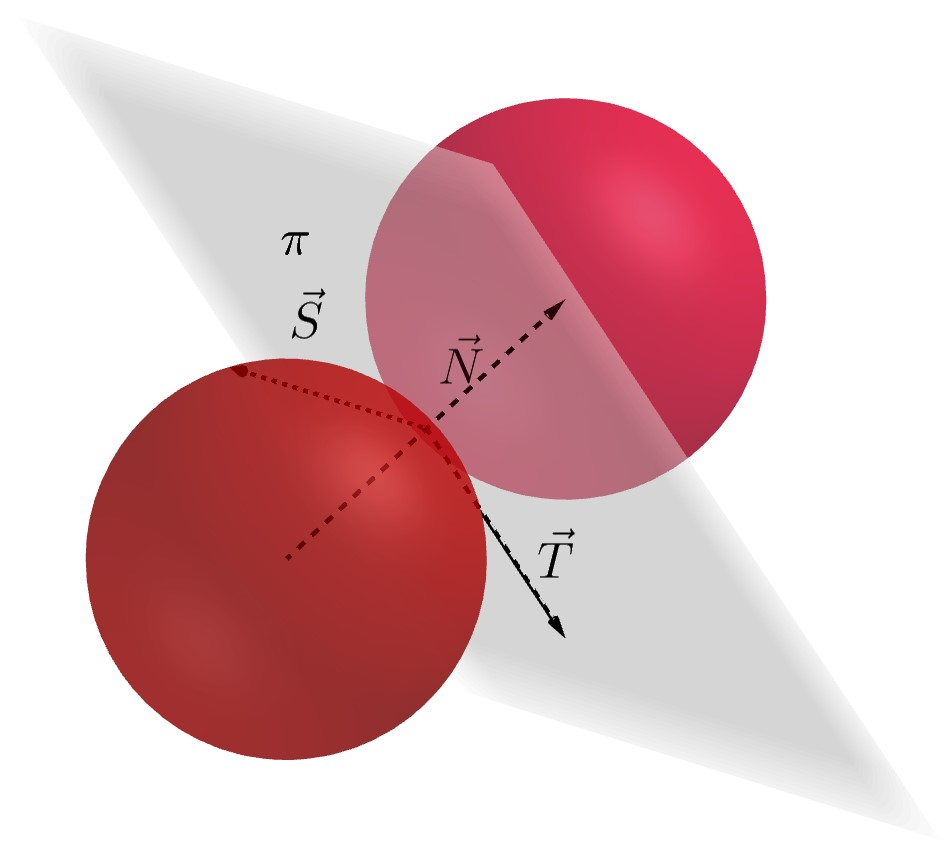
\includegraphics[width=4cm]{tcc/img/colisao_corrigida.jpg}
    \caption{Colisão entre dois corpos, plano tangente $\vet \pi$ e versores.}
    \label{fig:colisao-3d}
\end{figure}

Para obter os versores geradores do plano, basta tomar, por exemplo, os vetores
\begin{equation*}
    \vet T = \dfrac{(n_3, n_3,-n_1 - n_2)}{\norma{(n_3, n_3,-n_1 - n_2)}},
    \quad
    \vet S = \dfrac{\vet N \times \vet T}{\norma{\vet N \times \vet T}},
\end{equation*}
como na figura \ref{fig:colisao-3d}. Observe que $\vet T$ não é bem definido, uma vez que $n_1 = -n_2$ e $n_3 = 0$ gera $\vet T = \vet 0$. Na ocorrência desse caso, uma solução possível é utilizar outro vetor $\vet T$:
\begin{equation*}
    \vet T = \dfrac{(-n_2, n_1, 0)}{\norma{(-n_2, n_1, 0)}}.
\end{equation*}
Supondo que não ocorrem colisões reais, isto é, que $\vet N \neq \vet 0$ (o que, numericamente, é uma suposição válida), definimos $\vet S$ da mesma forma e o método que segue se mantém.

Com isso, as velocidades podem ser decompostas em relação ao plano tangente e em relação ao vetor normal:
\begin{align*}
    \vet v_1 &= \vet v_1^{\vet \pi} + v_1 \vet N,
    \\
    \vet v_2 &= \vet v_2^{\vet \pi} + v_2 \vet N.
\end{align*}

Uma vez que o sistema não contém rotações individuais, em uma colisão não há forças atuando nas direções do plano tangente, então a única alteração se dá nas componentes normais. Sendo $v_1'$ e $v_2'$ as novas velocidades normais, a colisão ser perfeitamente elástica implica na conservação do momento linear total e da energia cinética:
\begin{equation}\label{eq:colisoes_conservacao}
    \begin{cases}
        m_1 v_1 + m_2 v_2 = m_1 v_1' + m_2 v_2', \\
        m_1 v_1^2 + m_2 v_2^2 = m_1 v_1'^2 + m_2 v_2'^2.
    \end{cases}
\end{equation}

Do sistema de equações (\ref{eq:colisoes_conservacao}), decorre que
\begin{align*}
    v_1' &= \dfrac{v_1 (m_1 - m_2) + 2 m_2 v_2}{m_1 + m_2}, \\
    v_2' &= \dfrac{v_2 (m_2 - m_1) + 2 m_1 v_1}{m_1 + m_2}.
\end{align*}

Dessa forma, as novas velocidades após a colisão são:
\begin{align*}
    \vet v_1' = \vet v_1^{\vet \pi} + v_1' \vet N, \\
    \vet v_1' = \vet v_1^{\vet \pi} + v_1' \vet N.
\end{align*}

\begin{figure}[H]
    \centering
    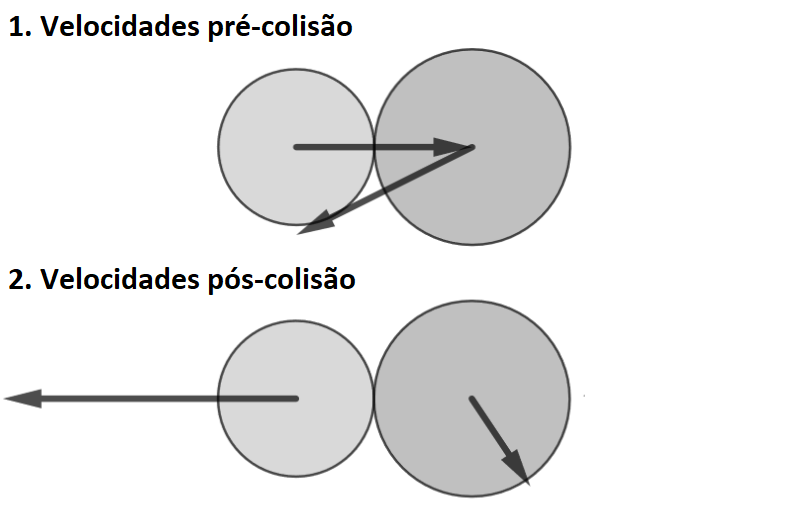
\includegraphics[width=8cm]{img/colisao_exemplo.png}
    \caption{Exemplo de colisão. Os tamanhos diferentes indicam massas diferentes.}
    \label{fig:colisao_exemplo}
\end{figure}

Na figura \ref{fig:colisao_exemplo} tem-se um exemplo de colisão entre dois corpos com massas diferentes. Como esperado, um corpo de massa menor sai da colisão com mais velocidade (e com sentido oposto), enquanto um de massa maior sai com menos velocidade (e com componente normal também no sentido oposto).

\section{Estabilidade}
% Falar um pouco da estabilidade e das ideias do momento de dilatação talvez. A princípio usar o capítulo do Volchan.

A principal motivação da última subseção foi obter uma forma conservativa de estender soluções do PNCG que são ``interrompidas''. Essa interrupção é, no sentido matemático, uma singularidade na órbita, o que limita o intervalo maximal para um tempo finito. O caso mais simples de interrupção é justamente uma colisão entre dois ou mais corpos.

\begin{definition}[Colisão]
    Diz-se que ocorre uma colisão no instante $t^*$ se cada $\vet q_j(t)$ tem limite finito quando $t \to t^*$, no sentido de que para algum $i \neq k$, $\vet q_i(t^*) = \vet q_k(t^*)$. Se para todo $i,k=1,2,...,N$ tem-se que $\vet q_i(t^*) = \vet q_k(t^*)$, então tem-se um \textbf{colapso total}.
\end{definition}

Apesar de ser uma exceção, o colapso total ocorre em situações interessantes para este trabalho. Decorre do teorema \ref{teorema:distanciamento} que se ele ocorre em algum instante $t = t^*$, então ele ocorre na origem. Para isso, basta ver pela definição \ref{def:momento_inercia} que $I(t^*) = 0$, então $q_{max} = 0$. Além disso, uma colisão total só ocorre em tempo finito.

\begin{proposition}
    Se ocorre o colapso total em $t=t^*$, então $t^* < +\infty$.
\end{proposition}
\begin{Proof}
    Suponha que $t^* = +\infty$. Como o colapso total ocorre na origem,
    \begin{equation*}
        \lim_{t \to +\infty} V(\vet q(t)) = - \infty
        \Rightarrow
        \lim_{t \to +\infty} \ddot I(t) = +\infty
    \end{equation*}
    através da identidade de Lagrange-Jacobi. Assim, existe $t_1 > 0$ de modo que para todo $t > t_1$ vale que $\ddot I(t) \geq 1$. Então:
    \begin{equation*}
        I(t) \geq \frac{1}{2} t^2 + c_1 t + c_2,
        \Rightarrow
        \lim_{t \to +\infty} I(t) = +\infty,
    \end{equation*}
    o que é uma contradição.
\end{Proof}

Outro ponto é que só ocorre o colapso total dentro de uma hipersuperfície específica do espaço de fases.

\begin{theorem}[Sundman-Weierstrass]
    Se ocorre o colapso total, então $\vet J = \vet 0$.
\end{theorem}

A demonstração pode ser encontrada em \citep[62-63]{Volchan:2007}. Um resultado importante também de Sundman é que se $\vet J \neq 0$, então não ocorrem colisões triplas. Na prática, através da regularização das colisões binárias, a solução de um problema com $\vet J \neq 0$ pode ter intervalo maximal estendido para toda a reta.

Nesse momento, qualquer definição de ``estabilidade'' das órbitas deve supor que não ocorre o colapso total, mas isso ainda não é suficiente. Um critério mais bem-definido proposto por Volchan é: para todo $i \neq j$ e todo $t \in \R$ e para uma constante $K > 0$,
\begin{enumerate}
    \item $r_{ij} \neq 0$;
    \item $r_{ij} \leq K$.
\end{enumerate}
Isto é, o sistema não só não cai sobre si mesmo, como também se mantém confinado em um cilindro de raio $K$. No caso de $\vet P = 0$, o sistema se encontra parado, então a restrição corresponde a uma esfera de raio $K$. Sistemas periódicos, por exemplo, atendem a essa propriedade.

De forma geral, Jacobi propôs uma condição necessária \citep[65]{Volchan:2007}.

\begin{theorem}[Critério de estabilidade de Jacobi]
    Uma condição necessária para que a solução seja estável é que a energia total seja negativa.
\end{theorem}
\begin{Proof}
    Como comentado anteriormente, se a energia é não-negativa então $I$ assume formato côncavo e é limitado inferiormente. Assim, $\lim_{t \to \infty} I(t) = +\infty$, então o tamanho do sistema não é limitado.
\end{Proof}

Para $N=2$, a condição é suficiente. Porém, isso não se estende para $N \geq 3$. Ainda assim, é possível obter outra condição necessária a partir da relação de Lagrange-Jacobi, ao que se denomina usualmente por \textbf{teorema do virial}.

\begin{theorem}[Teorema do virial]\label{teorema:virial}
    Uma condição necessária para que um sistema seja limitado é que
    \begin{equation*}
        \langle T \rangle_\tau = - \frac{1}{2} \langle V \rangle_\tau.
    \end{equation*}
\end{theorem}
\begin{Proof}
    O operador $\langle \cdot \rangle_\tau$ corresponde à média temporal no intervalo $[0, \tau]$. Pela identidade de Lagrange-Jacobi,
    \begin{equation*}
        \left\langle \der{D}{t} \right\rangle_{\tau}
        = 2 \langle T \rangle + \langle V \rangle.
    \end{equation*}
    Se um sistema é limitado então o momento de dilatação $D$ é limitado, e, uma vez que
    \begin{equation*}
        \left\langle \der{D}{t} \right\rangle_{\tau}
        = \frac{1}{\tau} \int_0^\tau \der{D}{t} dt = \dfrac{D(\tau) - D(0)}{\tau},
    \end{equation*}
    então
    \begin{equation*}
        \lim_{\tau \to \infty} \left| \left\langle \der{D}{t} \right\rangle_{\tau} \right| \leq \lim_{\tau \to \infty} \dfrac{D_{max} - D_{min}}{\tau} = 0.
    \end{equation*}
    Assim, vale $\langle T \rangle_\tau = - \frac{1}{2} \langle V \rangle_\tau$.
\end{Proof}

É possível estimar uma região do espaço em que vale o equilíbrio (de virial). Considere $N$ partículas dispostas com distância média $R_V$ com massa média $\bar m = M / N$, para $M = \sum_{a=1}^N m_a$. Temos que:
\begin{equation*}
    V = - G \sum_{a < b} \dfrac{m_a m_b}{r_{ab}}
    \approx - G \sum_{a<b} \bar m^2 \dfrac{1}{R_V}
    = - G \dfrac{M^2}{N^2} \dfrac{N (N-1)}{2 R_V}
    = - G \dfrac{M^2}{2 R_V} \dfrac{N-1}{N}.
\end{equation*}
Para $N$ grande, temos que
\begin{equation}\label{eq:raio_virial}
    V \approx - \dfrac{G M^2}{2 R_V}
    \Rightarrow
    R_V \approx \dfrac{G M^2}{2 |V|}.
\end{equation}

Tal $R_V$ é chamado \textbf{raio de virial}. A busca por sistemas estáveis deve começar por sistemas com energia negativa e para os quais valem o teorema do virial, e o raio de virial é útil nesse sentido. Isso é utilizado na geração de valores iniciais na seção \ref{subsection:condicoes_aarseth}, com as condições iniciais propostas por \citep{aarseth_gravitational_2003}. 

Também pode ser razoável supor que o momento angular total seja não nulo se o propósito for buscar estabilidade com mais facilidade, embora isso não seja condição necessária.

\section{A Dinâmica de Formas}\label{secao:dinamica_de_formas}
A Dinâmica de Formas (SD, do inglês \textit{Shape Dynamics}) é uma teoria de gravitação baseada em \textit{relacionalismo}, isto é, os conceitos absolutos de \textit{espaço} e de \textit{tempo} são suprimidos para basear a física na relação entre os objetos em questão - no caso do PNCG, a relação entre os corpos.

Embora seja um modelo alternativo de gravitação, foi a partir dela que começamos o estudo do PNCG como um todo, através do artigo \cite{Barbour2014_identification}. Por isso, apresentamos nesta seção uma breve introdução à versão quantizada (em massas pontuais) da SD e alguns de seus resultados qualitativos, que na seção \ref{secao:simulacao_dinamica_de_formas} são revisitados e podem ser visualizados através de simulações numéricas.

Nesta seção, algumas demonstrações foram omitidas tendo em vista facilitar a leitura do texto. Estas se encontram no Apêndice \ref{apendice:demonstracoes_dinamica_de_formas}. Além disso, as referências utilizadas encontram-se citadas no texto, mas as principais são o artigo mencionado, \cite{barbour2013_gravitationaloriginarrowstime} e \cite{Barbour2014_solution}.

%%%%%%%%%%%%%%%%%%%%%%%%%%%%%%%%%%%%%%%%%
\subsection{Contextualização e motivação}

O objetivo da Dinâmica de Formas é fornecer um modelo de gravitação que comporte a compreensão mecânica do físico e filósofo Ernst Mach (1838-1916), na qual apenas as relações inter-partícula são \textit{reais}. Para o problema de N-corpos em $\R^{3N}$, tomamos o quociente pelas translações e rotações euclidianas, obtendo o \textit{espaço de configurações relativas} (ECR) machiano, de $3N-6$ dimensões, o que remove as posições e orientações absolutas. Mais ainda, é preciso quocientar o ECR também em relação a \textit{dilatações}, para remover qualquer influência de escalas. Nisso, obtemos o \textit{espaço de formas} $S$ com $3N-7$ dimensões. 

Observe que ao quocientar $\R^{3N}$ pelas translações, a mecânica vigente ainda é a mecânica newtoniana, uma vez que o potencial newtoniano é invariante sob translações. Já para rotações, a situação não é a mesma, sendo o momento angular um elemento crucial de subsistemas fechados do universo (como o Sistema Solar). O modelo, então, se baseia no pressuposto de que não há rotação global no universo, mas somente rotações locais de subsistemas \citep[264]{Barbour2012_sd_introduction}.

Nessa situação, se torna aplicável um princípio que, embora não tenha sido enunciado diretamente por Mach, decorre de sua filosofia \citep[139]{Assis:1998}, que é chamado de \textit{princípio de Mach} ou \textit{de Mach-Poincaré}:

\begin{definition}[Princípio de Mach-Poincaré]
    A especificação de um ponto e uma direção (\textbf{forma forte}) ou de um ponto e um vetor tangente (\textbf{forma fraca}) no espaço de formas $S$ determinam a evolução em $S$ de forma única. \citep[31]{Barbour2014_kepler_mach}
\end{definition}

É fato importante que como um modelo de gravidade aplicável, existe uma interseção entre a Dinâmica de Formas e a Relatividade Geral, ocorrendo quando a Relatividade Geral comporta o Princípio de Mach-Poincaré: universos espacialmente fechados (\citealp[157]{Einstein:1981}; \citealp[258]{Barbour2012_sd_introduction}).

De toda forma, há diversas consequências da SD que são interessantes para a física, desde o próprio modelo de gravitação até implicações para uma gravidade quântica \citep{Barbour2012_sd_introduction}. Para este trabalho, o que interessa é a formulação de setas do tempo relacionais, uma forma de observar a evolução de sistemas de N-corpos baseada somente no próprio sistema.

%%%%%%%%%%%%%%%%%%%%%%%%%%%%%%%
% PRIMEIRO, PRECISO FALAR DO POR QUE QUERER SETAS DO TEMPO
% - MUITOS QUEREM DESCREVER A EVOLUÇÃO UTILIZANDO A ENTROPIA. O CONCEITO ORIGINAL NÃO FAZ SENTIDO PARA O PNCG, POIS A GRAVIDADE É DOMINANTE, O UNIVERSO NÃO TEM PAREDES E UM VOLUME GLOBAL FAZ ENTENDER QUE EXISTE ALGO MAIOR PARA REFERENCIAR.
Uma seta do tempo é um observável que não apenas caracteriza a evolução de um sistema dinâmico, mas também fornece uma orientação, no sentido de determinar o que é \textit{passado} e o que é \textit{futuro}. Na física, a maioria das discussões de setas do tempo se baseia no crescimento da entropia, uma medida de ``dispersibilidade'' de um sistema. Porém, no caso de sistemas puramente gravitacionais e fechados, a entropia como seta do tempo é uma escolha bastante questionável por algumas razões. Por exemplo, a conceitualização original de entropia se baseia em partículas fechadas em um espaço confinado e em um volume total do espaço de fases; ambas as bases não se encaixam ao Universo enquanto um sistema máximo no qual a gravidade é a força dominante.

% - A IDEIA ENTÃO É ABSTRAIR TODAS AS ESTRUTURAS EXTERNAS DA DINÂMICA DO PROBLEMA. NO PNCG, SÃO A POSIÇÃO, ORIENTAÇÃO E TAMANHO EM UM REFERENCIAL INERCIAL E UM TEMPO EXTERNO. UMA HISTÓRIA DINÂMICA É UMA CURVA UNPARAMETRIZED EM S. AS EQUAÇÕES DE MOVIMENTO DO PNCG SÃO SIMETRICAS NO TEMPO, ENTÃO NÃO DEFINEM UMA ORIENTAÇÃO EM C. TAMBEM POR ISSO, ENTROPIA E OUTRAS SETAS NÃO FAZEM SENTIDO.

% - UMA SETA DIGNA ENTÃO PRECISA TER ORIGEM EM UMA ASSIMETRIA DENTRO DO ESPAÇO S

Voltando ao enunciado sobre o princípio de Mach, o que realmente caracteriza a dinâmica do PNCG está no espaço $S$. Porém, as equações de movimento de Newton são simétricas no tempo, e portanto incapazes de fornecer uma orientação para a evolução de uma órbita em $S$. Assim, uma seta do tempo para o PNCG precisa ser caracterizada por alguma assimetria dentro do próprio espaço de formas.

% - COMO A ESCALA (DEGREES OF FREDOM) É UNICA E TEM DIMENSÕES, DEPENDENDO DE UMA ESCALA EXTERNA DEFINIDA, É PRECISO QUE AS SHAPE DOF NÃO TENHAM ESSE PROBLEMA. ATRAVÉS DE UMA DEPARAMETRIZAÇÃO, TRANSFORMAMOS A VARIÁVEL DE ESCALA (R) EM UM HAMILTONIANO (LOG R) E O SEU MOMENTO CONJUGADO MONÓTONO (D) NO PARÂMETRO DE EVOLUÇÃO (t). RESTA O MENOR CONJUNTO DE VARIÁVEIS NECESSÁRIAS PARA DESCREVER O UNIVERSO OBJETIVAMENTE.

\subsection{Eliminação da escala}
Uma questão sobre o PNCG é que o sistema comporta escalas. No entanto, já foi apresentado que através do Teorema \ref{teorema:similaridade_dinamica} é possível ignorar a escala, uma vez que aplicar um redimensionamento anisotrópico sobre uma trajetória fornece um conjunto de trajetórias com dinâmicas iguais a menos da escala. Uma representação objetiva do problema precisa ser capaz de condensar esse conjunto infinito de trajetórias dinamicamente equivalentes em uma única órbita em $S$. 

Para isso, podemos utilizar a raiz quadrada do momento de inércia $R$, pois este representa um tipo de \textit{desvio padrão} do sistema. Nesse caso, é preciso balancear cada posição com relação a sua massa, aplicando a transformação:
\begin{equation}
    \vet \sigma_a = \dfrac{\sqrt{m_a}}{R} \vet q_a,
    \quad a = 1, 2, ..., N.
\end{equation}
Observe que $\vet \sigma_a$ é adimensional. Além disso, trata-se uma coordenada dentro de uma bola unitária espacial na origem de $S$, uma vez que, por exemplo, para $N=1$ tem-se:
\begin{equation*}
    \vet \sigma_a = \dfrac{\sqrt{m_a} \vet q_a}{\sqrt{m_a} \norma{\vet q_a}} = \dfrac{\vet q_a}{\norma{\vet q_a}},
\end{equation*}
e valores maiores de $N$ oferecem um denominador maior que o numerador.

Podemos obter momentos conjugados para as coordenadas $\vet \sigma_a$ e que atendem à expectativa relacional, de que só é possível estar em movimento se for em relação a outra partícula:
\begin{equation*}
    \vet \pi_a = \dfrac{R}{\sqrt{m_a} D_0} \vet p_a - \dfrac{D}{D_0} \vet \sigma_a, \quad \forall a = 1, ..., N,
\end{equation*}
onde $D$ é o momento de dilatação ($D = R \dot R $). De fato, um sistema de uma só partícula não tem movimento:
\begin{equation*}
    \vet \pi_a 
    = \dfrac{\sqrt{m_a} \norma{\vet q_a}}{\sqrt{m_a} D_0} \vet p_a - \vet q_a \cdot \vet p_a \dfrac{\vet q_a}{D_0 \norma{\vet q_a}}
    = \dfrac{1}{D_0} (\norma{\vet q_a} \vet p_a - \vet p_a \norma{\vet q_a}) 
    = \vet 0, \quad \text{ se } N = 1.
\end{equation*}
Vale ressaltar que o par de coordenadas projetadas $(\vet \sigma, \vet \pi)$ (chamadas a partir daqui de \textit{objetivas}) ainda não é invariante por rotações. No entanto, obter uma forma explícita e rotacionalmente invariante é difícil, além de pouco produtivo, uma vez que o momento angular comuta em Poisson com a função hamiltoniana. (\citealp[21]{barbour2013_gravitationaloriginarrowstime}; \citealp{Barbour2014_identification}). Além disso, como esperado, as coordenadas objetivas possuem propriedades que correspondem às invariâncias exigidas por uma dinâmica adimensional:
\begin{align}\label{eq:new_constraints}
    R_{\vet \sigma} = \sum_{a=1}^N \vet \sigma_a \cdot \vet \sigma_a = 1, \quad
    D_{\vet \sigma, \vet \pi} = \sum_{a=1}^N \vet \pi^a \cdot \vet \sigma_a = 0, \nonumber \\
    \vet \sigma_{cm} = \sum_{a=1}^N \sqrt{m_a} \vet \sigma_a = 0, \quad
    \vet \pi_{\Sigma} = \sum_{a=1}^N \sqrt{m_a} \vet \pi^a = 0.
\end{align}
A restrição $R_{\vet \sigma}$ força que o sistema seja unitário, pois o que está se fazendo na prática é normalizar $R$. A restrição $D_{\vet \sigma, \vet \pi}$ corresponde ao processo para $D$, representando a invariância da escala global. Já $\vet \sigma_{cm}$ corresponde à ausência de movimento do sistema como um todo, análogo à conservação do centro de massas. Por fim, $\vet \pi_{\Sigma}$ corresponde à invariância do momento total. A demonstração destas propriedades consta no Apêndice \ref{apendice:demonstracoes_dinamica_de_formas} (Proposição \ref{prop:new_constraints}).

Também é possível verificar que $(\vet \sigma, \vet \pi)$ são invariantes por escala, uma vez que comutam com $D$ e com $R$ no sistema de coordenadas original
\begin{equation}\label{eq:invariancia_por_escala}
    \{ f(D,R), \vet \pi_a \} = \{ f(D, R), \vet \sigma_a \} = 0,
\end{equation}
onde $f$ é um observável para $D$ e $R$ (Proposição \ref{prop:invariancia_por_escala})

% - COMO SABER QUE SAO R E D? PRECISO ENUNCIAR NOVAMENTE O MOMENTO DE INERCIA, R E D E ATRAVES DE LAGRANGE-JACOBI MOSTRAR QUE D É MONÓTONO. USANDO O PARENTESE DE POISSON, POSSO MOSTRAR QUE O D É O MOMENTO CONJUGADO MONOTONO DE LOG R, ENTÃO FAZ SENTIDO FAZER

\subsection{Evolução de um sistema adimensional e complexidade}
Uma vez que o sistema deixa de ter escala, sua evolução depende de um correspondente à evolução da escala no problema original. Nesse caso, o momento de dilatação $D$ pode ser interpretado como variável de evolução para $E \geq 0$, uma vez que $D$ é monótono (Teorema \ref{teorema:lagrange_jacobi}). Para descrever o sistema nessa situação, é necessário um hamiltoniano baseado em $R$ e com variável baseada em $D$ que gere translações. Para isso, embora $R$ não seja canonicamente conjugado a $D$, $\log R$ é (veja equação \ref{eq:poisson_coordenadas_canonicas}), pois
\begin{equation*}
    \{\log R, D \} 
    = \sum_{a=1}^{N} \derpar{\log R}{\vet q_a} \derpar{D}{\vet p_a} - \derpar{\log R}{\vet p_a} \derpar{D}{\vet q_a}
    = \sum_{a=1}^{N} \dfrac{1}{R^2} m_a \norma{\vet q_a}^2 
    = 1.
\end{equation*}
Dessa forma, tomando uma variável de tempo adimensional $\tau = D/D_0$ (considerando $D_0 \neq 0$), temos um hamiltoniano $\mathcal H = - \log{(R/R_0)} + const$.

Descrever a energia cinética desse novo sistema não é difícil. Podemos decompor a energia cinética original em duas partes, uma correspondente à \textit{dilatação} $T_d = \frac{1}{2} D^2 / R^2$ e outra correspondente à \textit{forma} $T_S = \frac{1}{2} D_0^2 K_S / R^2$, onde
\begin{equation*}
    K_S = \sum_{a=1}^{N} \vet \pi_a \cdot \vet \pi_a = \dfrac{2 R^2 T - D^2}{D_0^2},
\end{equation*}
pois
\begin{equation*}
    T_d + T_S
    = \dfrac{1}{2} \dfrac{D^2}{R^2} + \dfrac{D_0^2}{2 R^2} K_S
    = \dfrac{1}{2} \left( \dfrac{D^2}{R^2} + 2 T - \dfrac{D^2}{R^2} \right) = T.
\end{equation*}

% - MAS COMO VAMOS DESCREVER A DINAMICA AQUI? PRECISAMOS DE UMA FUNÇÃO POTENCIAL PRA COISA, E ELA PRECISA SER 1/r² PARA QUE {H, D} = 0. O QUE CARACTERIZA BEM A EVOLUÇÃO DO SISTEMA? BOM, TEMOS OS TAMANHOS: L_RMS (R/M) E L_MHL (-V/M). A RAZAO DISSO FORNECE UMA MEDIDA DE COMPLEXIDADE BEM LEGAL QUE É INTRINSECA EM S.

A energia potencial, por outro lado, exige mais atenção. Como queremos um sistema invariante por escala, precisamos que o potencial seja homogêneo de grau $-2$ \citep[5]{Barbour2013_scaleanomaly}. Por outro lado, observando o sistema original, há duas medidas que caracterizam a dinâmica entre os corpos: a \textit{raiz da média quadrática} $\ell_{rms}$:
\begin{equation*}
    \ell_{rms} := \dfrac{1}{M^{1/2}} R,
\end{equation*}
e o \textit{comprimento harmônico médio} $\ell_{mhl}$:
\begin{equation}
    \ell_{mhl} = \dfrac{M^2}{|V|}.
\end{equation}
O comprimento $\ell_{rms}$ é uma medida interessante para o sistema como um todo, uma vez que dominam as maiores distâncias entre os corpos. Por outro lado, $\ell_{mhl}$ é uma medida bastante caracterizada pelas menores distâncias entre os corpos, uma vez que é inversamente proporcional às distâncias.

Unindo a necessidade de um potencial com grau $-2$ com o que se sabe sobre as escalas, podemos definir a complexidade
\begin{equation}
    C_S := \dfrac{\ell_{rms}}{\ell_{mhl}} = \dfrac{1}{M^{3/2}} R |V|.
\end{equation}
Observe que, além de atender o desejado, também trata-se de uma medida adimensional, sendo portanto \textit{intrínseca} do espaço $S$.

\begin{figure}
    \centering
    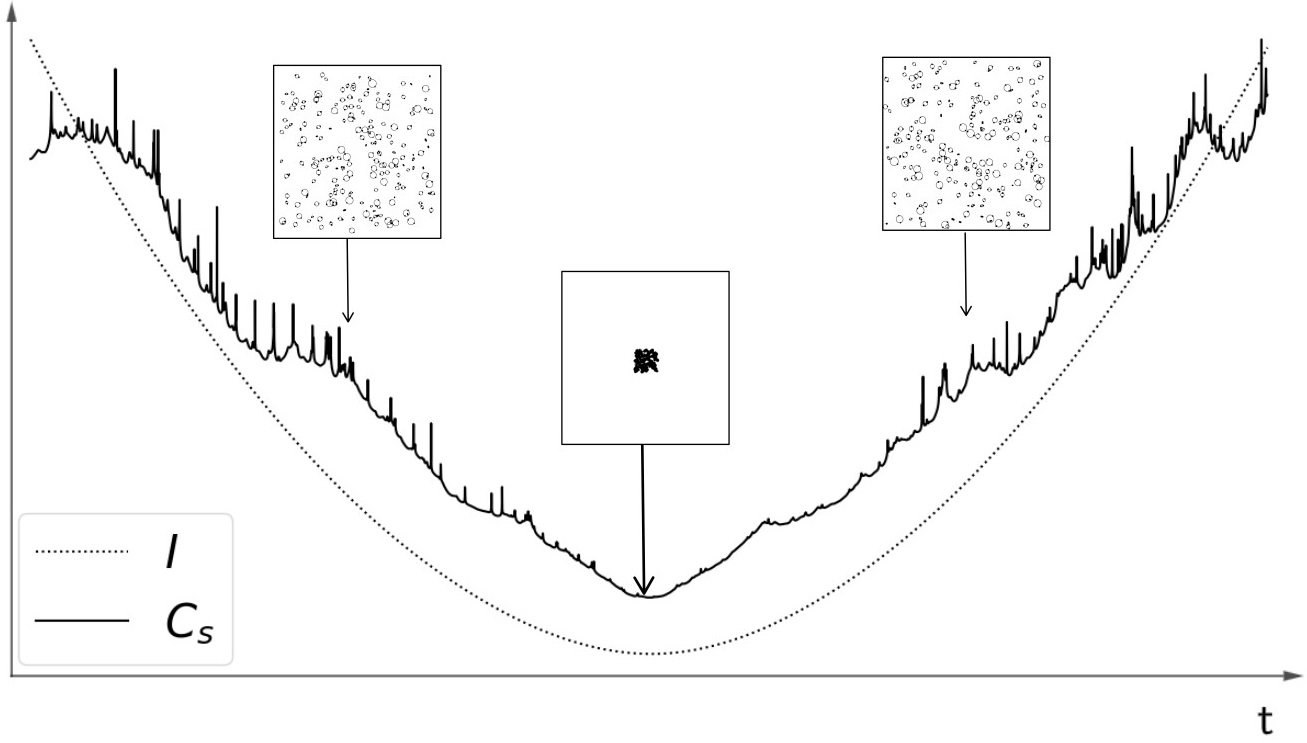
\includegraphics[width=0.5\linewidth]{tcc//img/complexidade.jpg}
    \caption{Visualização do espalhamento. O gráfico da complexidade corresponde a uma simulação de 100 corpos para $E=0$.}
    \label{fig:exemplo_espalhamento}
\end{figure}

% - A C_S É BOA POR DIVERSAS RAZÕES. ELA CARACTERIZA BEM TANTO A EVOLUÇÃO GERAL DO SISTEMA QUANTO O COMPORTAMENTO EM PEQUENA ESCALA. ELA CRESCER VARIANDO SIGNIFICA QUE A DISTANCIA ENTRE OS CORPOS FICA OSCILANDO.

% - SEGUNDO SAARI, PARA E = J = 0 O SISTEMA EVAPORA EM SUBSISTEMAS E CADA SUBSTISTEMA COMEÇA A CONVERGIR NO GERAL PARA CONSTANTES DE MOVIMENTO. QUANTO MAIS DIGITOS SAO CONSERVADOS EM UM SUBSISTEMA, MAIS ELE ESTÁ DISTANTE NA EVOLUÇÃO, ENTÃO A COMPLEXIDADE CARACTERIZA ISSO, A COMPLEXIDADE DO SISTEMA, O QUÃO ELE ESTÁ COMPLEXO. 

No caso em que $E=0$ e $\vet J = \vet 0$, \cite{Marchal1976} mostra que o sistema se divide em subsistemas (indexados por $\mathcal J$), e que cada subsistema, na medida em que se isola cada vez mais, desenvolve quantidade assintoticamente conservadas:
\begin{align*}
    E_{\mathcal J} (t) &= E_{\mathcal J} (\infty) + O(t^{-5/3}),\\
    \vet J_{\mathcal J} (t) &= \vet J_{\mathcal J} (\infty) + O(t^{-2/3}),\\
    \vet X_{\mathcal J} (t) / t &= \vet V_{\mathcal J} (\infty) + O(t^{-1/3}),
\end{align*}
onde $\vet X_{\mathcal J}$ é a distância do subsistema $\mathcal J$ ao centro de massas total do sistema e $\vet V_{\mathcal J} (\infty)$ é uma constante para a qual $\vet X_{\mathcal J}/t$ tende assintoticamente. Nessa situação, a complexidade caracteriza não apenas o distanciamento total entre os corpos, mas também as variações dentro dos subsistemas, como pode ser observado na figura \ref{fig:exemplo_espalhamento}, na qual $C_S$ cresce (indicando expansão do sistema) mas também varia (indicando as oscilações nos subsistemas).

% - ALEM DISSO, C_S É UM POTENCIAL DA FORMA DESEJADA, E UMA VEZ QUE R REMOVE A DEPENDENCIA DE ESCALA DE V_NEW, AS FORÇAS DERIVADAS DE C_S PODEM APENAS MUDAR A FORMA (SHAPE) DO SISTEMA, E NÃO O SEU TAMANHO. - LOG C_S TOMA O PAPEL DE POTENCIAL QUE ATRAI O SISTEMA TOWARDS MORE INHOMOGENEOUS SHAPES, E TEM MINIMOS E PONTOS DE SELA, MAS NAO MAXIMO GLOBAL.

\subsection{Equações de movimento no espaço de formas $S$}

Outro ponto para a complexidade como energia potencial do sistema é o fato de que $R$ remove a dependência da escala de $V$, então as forças derivadas de $C_S$ são capazes apenas de mudar a forma do sistema, e não o seu tamanho. A função $-\log C_S$ toma o papel de um potencial que leva o sistema para formas mais não-homogêneas.

% - COM ISSO EM MÃOS, AGORA DEFINIMOS AS NOVAS COORDENADAS E PODEMOS RE-ESCREVER O LOG R E OBTER UM HAMILTONIANO LEGAL MAS tau-DEPENDENTE. 

Com a decomposição da energia cinética e a nova energia potencial, agora é possível obter uma expressão para $\mathcal H$ em função de $\vet \sigma$ e $\vet \pi$. Isso é feito tomando em conta que
\begin{equation*}
    R^2 E - M^3 R C_S - \frac{1}{2} D^2 - \frac{1}{2} D_0^2 K_S = 0,
\end{equation*}
e então se $E = 0$ é possível obter uma expressão para $R$, e consequentemente para $\mathcal H$:
\begin{equation}\label{eq:hamiltoniano_tau_dependente}
    \mathcal H (\tau) = \log{(K_S + \tau^2)} - \log{C_S}.
\end{equation}

Para esse hamiltoniano $\tau$-dependente, obtemos um conjunto de equações de Hamilton também $\tau$-dependentes:
\begin{equation}
    \der{\vet \sigma_a}{\tau} = \dfrac{2 \vet \pi_a}{K_S + \tau^2},
    \quad
    \der{\vet \pi_a}{\tau} = \derpar{\log C_S}{\vet \sigma_a} - \dfrac{K_S}{K_S + \tau^2} \vet \sigma.
\end{equation}

% - PODEMOS ENTÃO INTRODUZIR LAMBDA = LOG TAU E DIVIDIR PI POR D, OQ FORNECE UM HAMILTONIANO AUTONOMO QUE DESCREVE METADE DO SISTEMA. POREM, AS EQUAÇÕES AGORA POSSUEM UMA FRICÇÃO NÃO CANONICA -OMEGA QUE ESPONTANEAMENTE DISSIPA O MOMENTO ADIMENSIONAL. ISSO JUNTO DO FATO DO POTENCIAL -LOGCS NAO TER MINIMO LOCAL EXPLICA POR QUE CS CRESCE SECULARMENTE (PORQUE É O OPOSTO DE UM POTENCIAL DE UM SISTEMA COM FRICÇÃO)
\subsection{A escala como fricção em $S$}

A dependência temporal de $\mathcal H$ pode ser eliminada através de uma mudança de coordenadas. Tomando $\lambda = \log \tau$ e definindo $\vet \omega_a = \vet \pi^a / \tau$ como um novo momento conjugado adimensional, obtemos um novo hamiltoniano $H_0$ dado por
\begin{equation}
    H_0 = \log\left(\sum_{a=1}^{N} \vet \omega^a \cdot \vet \omega^a + 1\right) - \log C_s,
\end{equation}
O custo dessa transformação é obter um conjunto não canônico de equações de movimento:
\begin{equation}
    \der{\vet \sigma_a}{\lambda} = \derpar{H_0}{\vet \omega_a},
    \quad
    \der{\vet \omega_a}{\lambda} = - \derpar{H_0}{\vet \sigma_a} - \vet \omega_a.
\end{equation}

O termo $\vet \omega_a$ na equação do momento é um tipo de  \textit{fricção sobre as equações}, indicando que existe dissipação. Dinamicamente, isso indica que o distanciamento dos subsistemas, refletido no problema original no aumento da escala, é refletido em $S$ por uma desaceleração na medida em que se aproxima do bordo da esfera unitária, ao ponto de, no limite, ter velocidade nula. Isso caracteriza uma assimetria sobre as trajetórias em $S$.

Por outro lado, o sistema com $H_0$ indica mais nitidamente o comportamento do sistema. Uma vez que o movimento é regido por um potencial $-\log C_S$ sujeito a fricção linear, $C_S$ deve crescer indefinidamente no problema com integrais primeiras nulas. Além disso, a dinâmica para $H_0$ tem um início delimitado, com um passado distante sendo o ponto-limite em que $D=0$. Isso reforça que $C_S$ possui um mínimo global, denominado \textit{Ponto de Janus}, a partir do qual o sistema pode evoluir em duas direções ($D > 0$ e $D < 0$), sendo cada direção orientada pelo crescimento de $C_S$. Dessa forma, $C_S$ caracteriza uma seta do tempo para o PNCG.

% - SETAS. DESCREVEMOS O PNCG COMO UM SISTEMA DINAMICO NO ESPAÇO DE FORMAS CUJO MOVIMENTO É REGIDO POR UM POTENCIAL -LOG CS SUJEITO A FRICÇÃO LINEAR. NESSE CASO, TEMOS UMA ORIENTAÇÃO PARA O SISTEMA: A DIREÇÃO EM QUE A ESTRUTURA, MEDIDA POR CS, CRESCE.
\subsection{Observações}

O caso em que $\vet J = 0$ mas $E > 0$, porém, é particularmente interessante, pois grande parte da teoria apresentada permanece válida. No lugar do $\mathcal H$ de \ref{eq:hamiltoniano_tau_dependente}, obtemos um hamiltoniano diferente:
\begin{equation*}
    \mathcal H = \log{\left[ C_S + \sqrt{C_S^2 + \frac{1}{2} \epsilon (K_S + \tau ^2)} \right]},
    \quad
    \epsilon = E D_0^2.
\end{equation*}
Nesse caso, o princípio de Mach-Poincaré falha, uma vez que é necessário especificar $\epsilon \tau^2$, mas a dinâmica continua invariante por escala e totalmente adimensional com uma variável monótona independente. No entanto, a evolução final fica mais firmemente estabelecida: o potencial é dependente do tempo e é idêntico a $C_S$ somente no instante inicial, apresentando um comportamento dissipativo com o tempo. Assintoticamente, o sistema congela.

% - QUESTÕES. AS EQUAÇÕES OBJETIVAS EM S MUDAM SE E E J NAO SAO NULOS. NESSE CASO O UNIVERSO CORRESPONDE NÃO APENAS A S MAS A ESTRUTURAS EXTERNAS. POREM, O CASO E = J = 0 BATE COM A ESTRUTURA BÁSICA DO CLOSED-SPACE VACUUM GR E PROVIDENCIA UM MODELO OK PRO UNIVERSO. ALEM DISSO, CS PODE PARECER UM CASAMENTO ARTIFICIAL SÓ PARA DAR ALGO ADIMENSIONAL, MAS O QUE É ARTIFICIAL É SEPARAR R DE V_NEW.
Outros valores para as integrais primeiras podem ser considerados. No entanto, se $E$ e $\vet J$ não são nulos as trajetórias não se resumem a $S$, mas dependem de outras estruturas externas. Uma vez que, como mencionado, o caso com integrais primeiras nulas quando estendido para a versão relativística da Dinâmica de Formas coincide com a Relatividade Geral, são valores razoáveis para se assumir como hipótese.

Outro ponto é sobre o processo de obtenção de $C_S$. Embora soe artificial a definição da complexidade como feita, $C_S$ é adimensional e caracteriza intrinsecamente a dinâmica do PNCG, sendo portanto um valor que de fato \textit{existe} para o problema. Por outro lado, separar a evolução do sistema entre $R$ e $V$, entre os corpos distantes e os corpos próximos, é o que se poderia chamar de artificial.

Assim, para além de um modelo interessante, a Dinâmica de Formas foi introduzida neste trabalho primeiro como motivação, e segundo como uma fonte de propriedades qualitativas do PNCG que podem ser visualizadas através de simulações numéricas. Na seção \ref{secao:simulacao_dinamica_de_formas} nós retomamos e aplicamos numericamente um pouco do que foi apresentado nesta seção.


% Nesse sentido, para $E \geq 0$, como $D$ é monótono este pode ser usado como uma medida de tempo $\tau = D/D_0$, onde $D_0 = D(t_0)$.

% \begin{figure}
%     \centering
%     \includegraphics[width=0.5\linewidth]{tcc//img/complexidade1000.png}
%     \caption{N=1000, h=0.04, e=0.04, [-10³, 10³], verlet, 464s + 451s}
%     \label{fig:enter-label}
% \end{figure}
% \begin{figure}
%     \centering
%     \includegraphics[width=0.5\linewidth]{tcc//img/complexidade_1000_energia_0.png}
%     \caption{Enter Caption}
%     \label{fig:enter-label}
% \end{figure}

% \begin{figure}
%     \centering
%     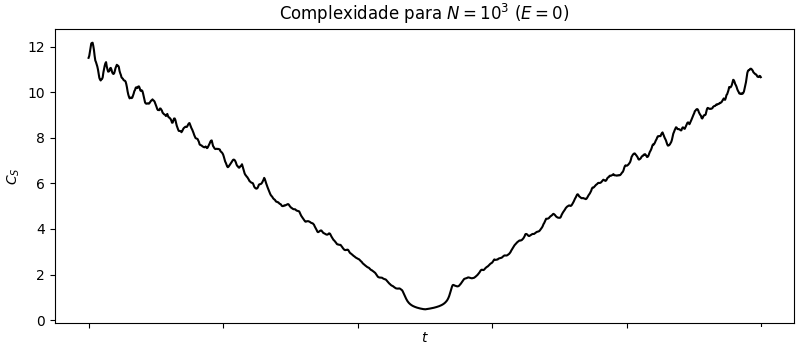
\includegraphics[width=0.5\linewidth]{tcc//img/complexidade_1000_nula.png}
%     \caption{Enter Caption}
%     \label{fig:enter-label}
% \end{figure}